% !TeX spellcheck = en_US
% !TeX root = ../build/road-to-scalability.tex
% !TeX TXS-program:compile = txs:///xelatex/[--shell-escape]



%%%%%%%%%%%%%%%%%%%%%%%%%%%%%%%%%%%%%%%%%%%%%%%%%%%%%%%%%%%%%%%%%%%%%%%%%%
\section{Introduction}
\textbf{Blockchain interoperability} refers to the ability of a blockchain to interchange data with other blockchains. Since the blockchain ecosystem has expanded rapidly in recent years, a large number of networks with different specific properties have emerged and interoperability has become a crucial consideration in blockchain design. Without interoperability, a network risks being isolated from the larger ecosystem and this fact has supposed an incentive to projects to engage the research and development of interoperability solutions. Multiple approaches have been implemented in order to solve the problem, each one of them with particular trade offs and underlying technologies. This document describes the solution implemented by the Polygon team to bring native interoperable properties to the Polygon zkEVM L2 network.




\section{The Bridge}
The bridge is an infrastructure component that allows migration of assets and communication between different layers. From the point of view of the user, they should be able to transfer an asset from one network to another without changing its value or its functionality, as well as being able to send data payloads between networks (\textbf{cross-chain messaging}).

For sake of simplicity, we will start the bridge description by defining exchanges between L1 and an L2 but our intention is to be general, that is, to enable exchanges between multiple layers LX and LY. This is why we call this subsystem the \textbf{LXLY bridge}. For the explanations, we will use three layers denoted as LX, LY and LZ as represented in Figure \ref{fig:lxlylz}.

\begin{figure}[H]
\centering
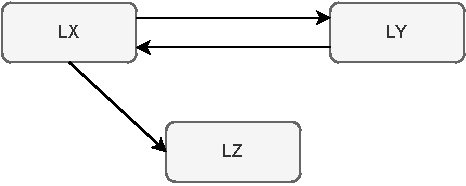
\includegraphics[width=0.6\textwidth]{\zkevmdir/figures/architecture/layer-communication/lxlylz.drawio}
\caption{Layered Architecture Example: Illustration of Two Top Layers (LX, LY) and a Bottom Layer (LZ).}
\label{fig:lxlylz}
\end{figure}







\section{Exchanging assets and messages}
The objective of the bridge component is to enable the exchange of both \textbf{assets} and \textbf{messages} (See Figure \ref{fig:assets-messages}). On the one hand, the term \textbf{asset} refers to any digital representation of value within the Ethereum blockchain. Ethereum supports two types of assets: \textbf{Ether (ETH)}, which is the native cryptocurrency of the network, and \textbf{Tokens}, including ERC-20 and ERC-721 tokens. On the other hand, a \textbf{message} refers to communication or interaction between two smart contracts, involving both data and a value (in ETH) transferred from the origin contract (the one initiating the message) to the specified destination contract. Within the zkEVM context, these messages entail the execution of a function \texttt{onMessageReceived} of some existing contract. This is what we call the \textbf{messaging mechanism} of the bridge.

\begin{figure}[H]
\centering
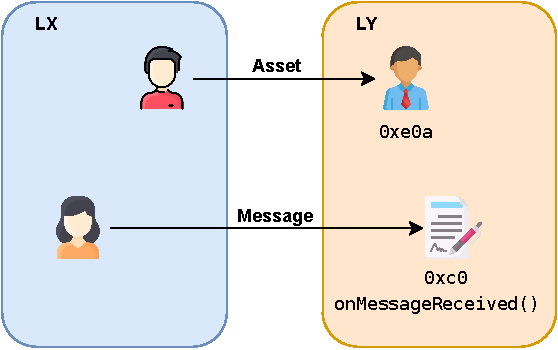
\includegraphics[width=0.4\textwidth]{\zkevmdir/figures/architecture/layer-communication/assets-messages.drawio}
\caption{The bridge component should be able to exchange both assets and messages.}
\label{fig:assets-messages}
\end{figure}

The core logic of the LXLY bridge is implemented in smart contracts. In particular, the main contract is called \texttt{zkEVMBridge.sol} that is deployed in any layer in which we want exchanging to be enabled. One of the design goals is that this smart contract \textbf{is exactly the same in all layers} (See Figure \ref{fig:bridge-claim-method}). This uniformity is intentional to maintain consistency in the logic whether exchanging assets or messages from a lower layer LY to an upper layer LX, or vice versa and hence externalizing the complexity associated with the layer position distinction from the core contract.

\begin{figure}[H]
\centering
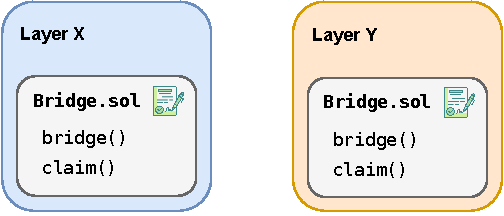
\includegraphics[width=0.5\textwidth]{\zkevmdir/figures/architecture/layer-communication/bridge-claim-method.drawio}
\caption{Uniform deployment of \texttt{zkEVMBridge.sol} in all layers ensures consistent handling of exchanges in the LXLY bridge's core logic.}
\label{fig:bridge-claim-method}
\end{figure}

The LXLY bridge follows a \textbf{bridge-claim model} (See Figure \ref{fig:lxly-exchange}). Let us suppose we are in the situation where some LX user wants to transfer an asset (or, alternatively, a message) to some LY user. In the origin layer LX, the source user sends a transaction to the \texttt{bridge()} function providing the destination network LY. From now on, transactions to the bridge function will also be known as \textbf{deposits}. Later on, in the destination layer LY, the user sends a transaction to the \texttt{claim()} function providing the origin network LX in order to claim the \textit{transferred} (we will explore the meaning of that later on) asset (or message). To maintain a record of exchanges across layers, within the \texttt{zkEVMBridge.sol} smart contracts we need a compact way of storing the information of calls to the bridge function. These data, often referred to as \textbf{exits} or \textbf{outgoing transmissions}.

\begin{figure}[H]
\centering
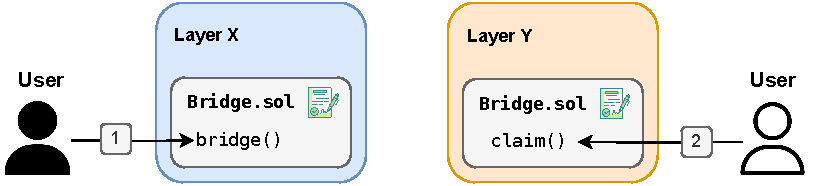
\includegraphics[width=0.7\textwidth]{\zkevmdir/figures/architecture/layer-communication/lxly-exchange.drawio}
\caption{LXLY bridge adopts a bridge-claim model for transferring assets and messages.}
\label{fig:lxly-exchange}
\end{figure}